\documentclass[11pt]{article}
\usepackage{fullpage,amsmath,amsfonts,mathpazo,microtype,nicefrac,graphicx}

% Set-up for hypertext references
\usepackage{hyperref,color,textcomp}
\definecolor{webgreen}{rgb}{0,.35,0}
\definecolor{webbrown}{rgb}{.6,0,0}
\definecolor{RoyalBlue}{rgb}{0,0,0.9}
\hypersetup{
   colorlinks=true, linktocpage=true, pdfstartpage=3, pdfstartview=FitV,
   breaklinks=true, pdfpagemode=UseNone, pageanchor=true, pdfpagemode=UseOutlines,
   plainpages=false, bookmarksnumbered, bookmarksopen=true, bookmarksopenlevel=1,
   hypertexnames=true, pdfhighlight=/O,
   urlcolor=webbrown, linkcolor=RoyalBlue, citecolor=webgreen,
   pdfauthor={Chris H. Rycroft},
   pdfsubject={Harvard AM205 (Fall 2017)},
   pdfkeywords={},
   pdfcreator={pdfLaTeX},
   pdfproducer={LaTeX with hyperref}
}
\hypersetup{pdftitle={AM205: Final Project}}

% Macro definitions
\newcommand{\N}{\mathbb{N}}
\newcommand{\Z}{\mathbb{Z}}
\newcommand{\Q}{\mathbb{Q}}
\newcommand{\R}{\mathbb{R}}
\newcommand{\B}{\mathbb{B}}
\newcommand{\mcL}{\mathcal{L}}
\newcommand{\p}{\partial}
\newcommand{\Trans}{\mathsf{T}}
\renewcommand{\vec}[1]{\mathbf{#1}}
\newcommand{\vx}{\vec{x}}
\newcommand{\vb}{\vec{b}}

\DeclareMathOperator{\rank}{rank}

\begin{document}
\section{Results and Discussions}
\subsection{Simple ODEs}
Overview
\break
Mathematics
\break
Results 
\break
Discussions


\subsection{Unstable, Periodic ODEs}


\subsubsection{Lotka-Volterra  2-species model}
Overview
\break

The Lotka-Volterra prey-predator equations are a pair of first-order, non-linear differential equations commonly used to describe the interactions between two species, the prey and predator.
\break

Mathematics
\break
The populations of the prey and predator can be described by the following equations:

    \begin{equation}
      \frac{dx}{dt} = ax - bxy
      \label{eq:LV1}
    \end{equation}
    
     \begin{equation}
      \frac{dy}{dt} = -cy + dxy
      \label{eq:LV2}
    \end{equation}
    

where
\begin{itemize}
\item $x$ is the density of prey
\item $y$ is the density predator
\item $t$ represents time
\item $a, b, c, d >0$ 
\end{itemize}

Eq.~\ref{eq:LV1} indicates that in the absence of a predator ($y = 0$), the prey would grow at a constant rate $a$, with the assumption that the prey have an unlimited food supply. The rate of predation upon the prey is assumed to be proportional to the rate at which the predators and the prey are present concurrently, represented by $bxy$. If either $x$ or $y$ is zero then no predation is possible.

Similarly, Eq.~\ref{eq:LV2} shows that in the absence of prey ($x = 0$), the density of predators would decrease at a constant rate $c$, due to natural death or emigration. This equation assumes that the predator population only preys upon the same species of prey identified in Eq.~\ref{eq:LV1}. $dxy$ represents the growth of the predator population[REF1].

The model assumes that throughout the process the external environment remains the same and none of the species is favored.[REF2]

Results 
\break

\begin{figure}
\centering
\includegraphics[width=0.7\textwidth]{LV_compare.png}
      \caption{Comparing across results using standard ODE solver from Scipy library versus using neural net solver, at initial parameters of $a = 1$, $b = 0.1, c = 1.5, d = 0.75$.\label{fig:LVFig}}
\end{figure}

From this plot we see that our neural net solver attains a close fit to the ODE solver. To enable us to evaluate the fit of the two functions in this system of ODEs, we propose taking an average of the RMSE, in this case we will have:

\begin{equation}
RMSE_{overall} = \frac{1}{2}[RMSE_{prey} + RMSE_{predator}]
\end{equation}

For this particular plot, the overall average RMSE is at $3.2$. It is found that while our proposed solver using neural net is able to provide a continuous function, the results tend to fluctuate highly. As such, we ran the same fitting over 100 times as shown in Fig. ~\ref{fig:perf_dist}. 38 of the 100 fittings result in relatively good fitting with average RMSE of less than 15.

\begin{figure}
\centering
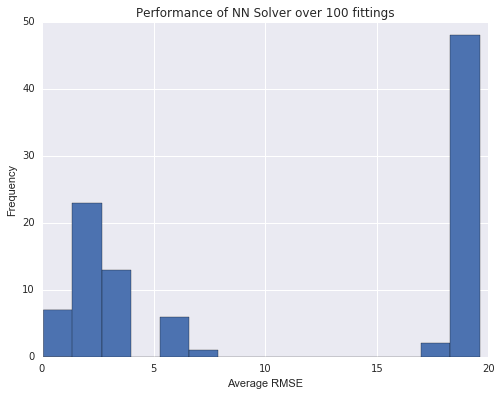
\includegraphics[width=0.7\textwidth]{perf_distribution.png}
      \caption{Running NN solver 100 times to see the performance histogram \label{fig:perf_dist}}
\end{figure}

Discussions

\subsubsection{Lotka-Volterra 3-species Model}
Extending to the 2-species model discussed earlier, we wish to model a linear three-species food chain where the lowest-level prey $x$ is preyed upon by a mid-level species $y$, which, in turn, is preyed upon by a top level predator $z$. An example of a three-species food chain is mouse-snake-owl [REF3].  

    \begin{equation}
      \frac{dx}{dt} = ax - bxy
      \label{eq:LV3}
    \end{equation}
    
     \begin{equation}
      \frac{dy}{dt} = - cy + dxy - eyz
      \label{eq:LV4}
    \end{equation}
    
     \begin{equation}
      \frac{dz}{dt} = - fz + gyz
      \label{eq:LV5}
    \end{equation}
where
\begin{itemize}
\item $a, b, c, d, e, f, g >0$ 
\item $a, b, c, d$ are as in the 2-species Lotka-Volterra equations
\item $e$ represents the effect of predation on species $y$ by species $z$
\item $f$ represents the natural death rate of species $z$ in the absence of prey
\item $g$ represents the reproduction rate of species $z$ in the presence of prey $y$
\end{itemize}

Results
\begin{figure}
\centering
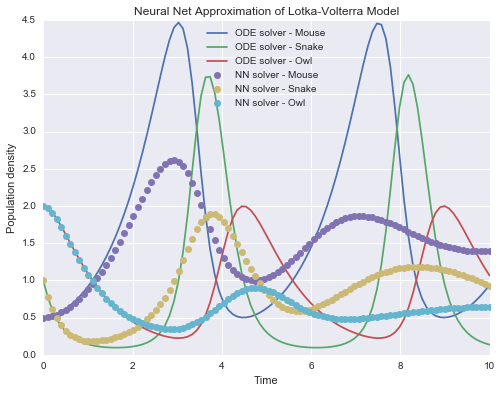
\includegraphics[width=0.7\textwidth]{LV_Compare_3_species.png}
      \caption{Comparing across results using standard ODE solver from Scipy library versus using neural net solver, at initial parameters of $a = b = c = d = e = f = g = 1 $.\label{fig:LVFig_3_species}}
\end{figure}

We can see that the performance is worse compared to the 2-species Lotka-Volterra model. 

\subsubsection{Van der Pol oscillator}
Overview

Van der Pol oscillator is a non-conservative oscillator with a linear spring force and a non-linear damping force.  [REF4] The equation is given by:
     \begin{equation}
      \frac{d^2x}{dt^2} - \mu(1-x^2)\frac{dx}{dt} + x = 0
      \label{eq:VDP}
    \end{equation}
    
Mathematics

Applying the Li\'enard transformation $y = x - \frac{x^3}{3} - \frac{1}{\mu}\frac{dx}{dt}$, the equation can be written as a system of ODE [REF5]:

     \begin{equation}
      \frac{dx}{dt} = \mu(x - \frac{1}{3}x^3 - y)
      \label{eq:LV4}
    \end{equation}
    
     \begin{equation}
      \frac{dy}{dt} = \frac{x}{\mu}
      \label{eq:LV5}
    \end{equation}
    
Results


\begin{figure}
\centering
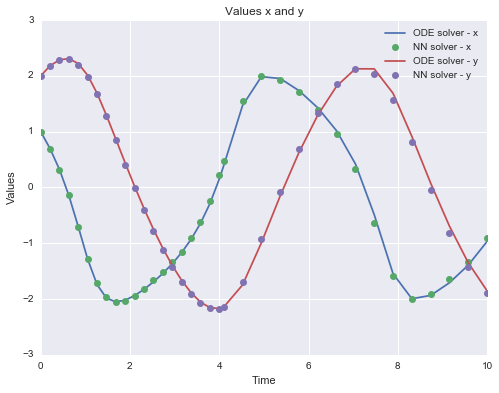
\includegraphics[width=0.7\textwidth]{VDP_non_uniform.png}
      \caption{Running NN solver with uneven spacing on time points. Average RMSE of 0.00238. \label{fig:VDP_non_uniform}}
\end{figure}


\begin{figure}
\centering
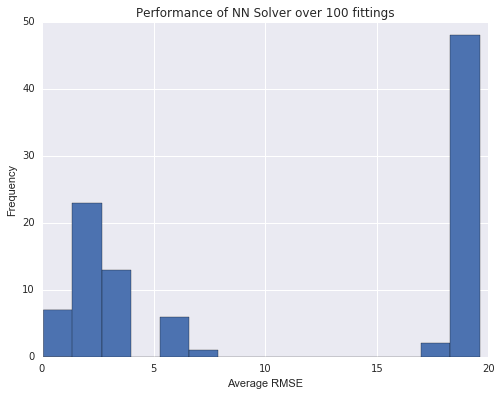
\includegraphics[width=0.7\textwidth]{perf_distribution.png}
      \caption{Running NN solver 100 times to see the performance histogram \label{fig:perf_dist}}
\end{figure}

Discussions


%1. https://en.wikipedia.org/wiki/Lotka-Volterra_equations
%2. http://www.math.harvard.edu/library/sternberg/slides/11809LV.pdf
%3. http://people.kzoo.edu/barth/math280/articles/3speciesLV.pdf
%4. http://www2.me.rochester.edu/courses/ME406/webexamp5/vanpol.pdf
%5. Kaplan, D. and Glass, L., Understanding Nonlinear Dynamics, Springer, 240–244, (1995).
\end{document}